\begin{frame}
\frametitle{Renderizzare Un Colore: Demo}
\begin{figure}[ht]
    \centering
    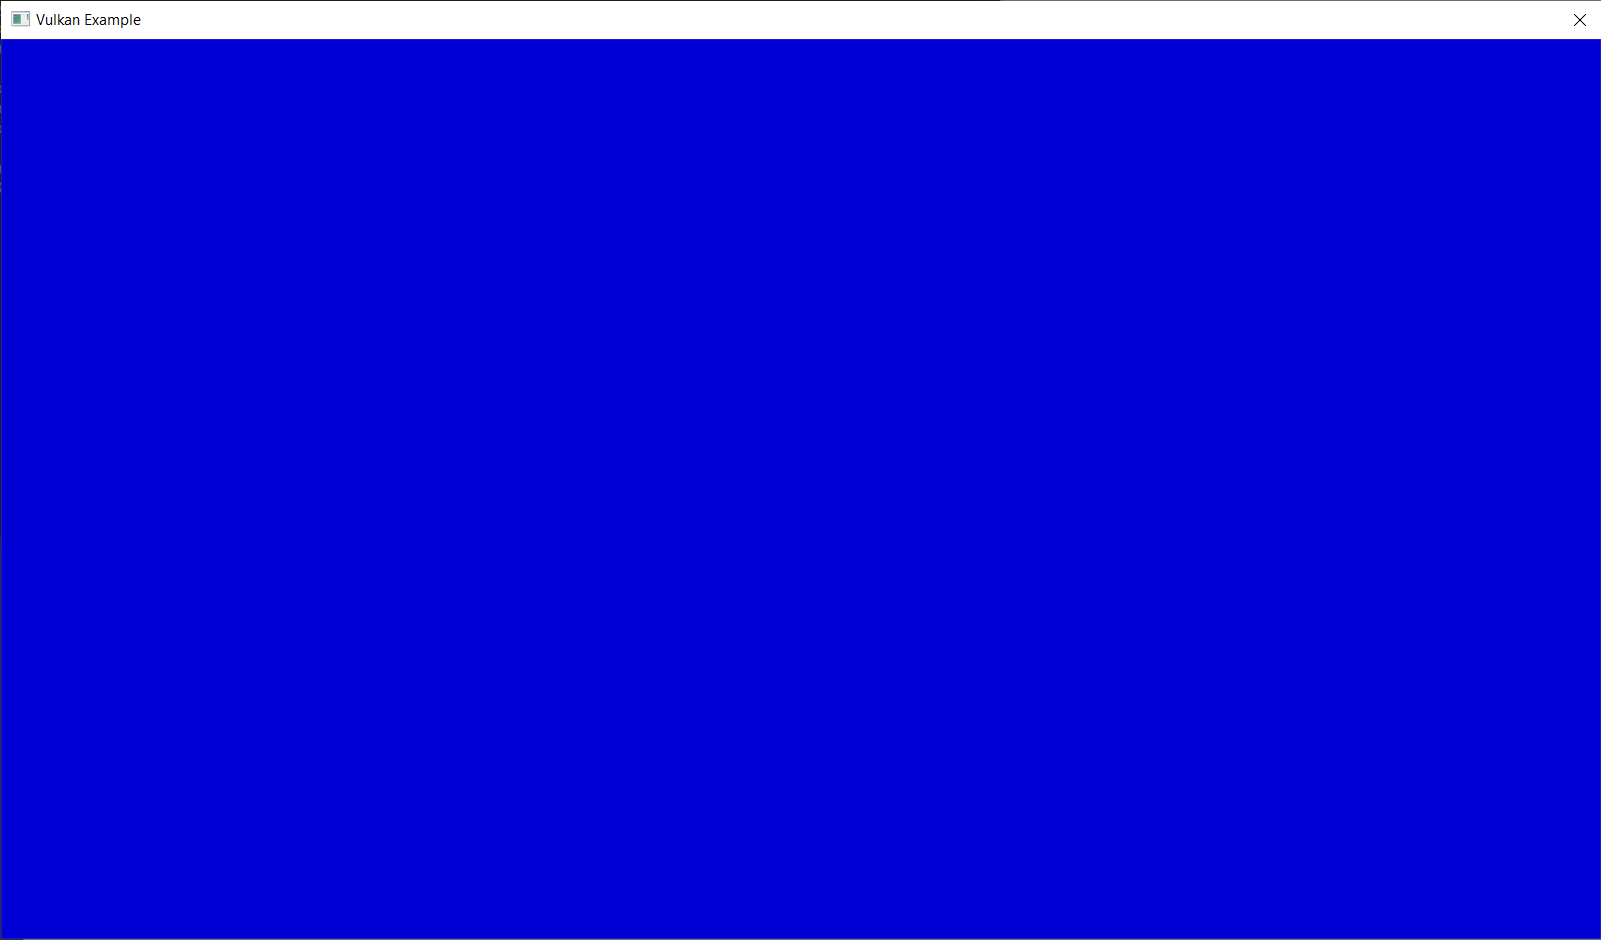
\includegraphics[scale=0.25]{images/SlidesClearWindow/ClearWindow.png}
\end{figure}
\end{frame}

\begin{frame}
\frametitle{Renderizzare Un Colore}

\begin{itemize}
\item Creazione di un render pass
\item Un render pass descrive gli attachment che vengono utilizzati durante il rendering
\item Un render pass raggruppa i comandi grafici in uno o più subpass in base a come e quali attachment utilizzano
\item Creazione di un framebuffer
\item Un reamebuffer è l'insieme di attachment utilizzati da un'istanza di un render pass
\item Creazione di un command buffer
\item Scrittura di comandi su un command buffer
\item Inviare un command buffer alla GPU
\item Presentare un'immagine sulla presentation surface
\end{itemize}
\end{frame}
